%\documentclass[12pt,a4paper,twocolumn,oneside,landscape]{article}
\documentclass[12pt,a4paper]{article}
%\usepackage{amsmath}
%\usepackage{amsfonts}
%\usepackage{amssymb}
%\usepackage{eurosym} 
\usepackage{graphicx}

\usepackage{wrapfig}
%\usepackage[latin1]{inputenc}
% D'après ce que j'ai lu, latin1 est pour Unix, tandis que ansinew est pour Window
\usepackage[utf8]{inputenc}
\usepackage{textcomp}
\usepackage[OT1, T1]{fontenc}
% lmodern remplace fontenc, résultation vachement mieux, mais des
% comportement bizarre avec \verb.
%\usepackage{lmodern}
%\usepackage{kpfonts}
\usepackage{mathpazo}
%\usepackage{mathptmx}
%\usepackage{helvet}
%\usepackage{emerald}
\usepackage{listings}




%\usepackage[francais]{babel}
\usepackage[frenchb]{babel}
\usepackage[colorlinks=true, urlcolor=blue, pdfhighlight =/O]{hyperref}
\usepackage[margin=2cm,columnsep=0.8cm,marginparwidth=1.5cm]{geometry}
    
% En-tete et pied de page doivent se faire ici, après {geometry}             
\usepackage{fancyhdr} \pagestyle{fancy}
\usepackage{lipsum, xcolor, lastpage}

\renewcommand{\headrulewidth}{.1px}
\renewcommand{\footrulewidth}{.1px}

\fancyhead{} % clear all header fields
\fancyhead[L]{\scriptsize{UHA/FST}}
\fancyhead[R]{\scriptsize{Licence 3 Info/MIAGE}}
\fancyhead[C]{\scriptsize{Examen Java du 5 mars 2012 (Yvan Maillot)}}

\fancyfoot{} % clear all footer fields
\fancyfoot[L]{\scriptsize{Dur�e 2h}}
\fancyfoot[C]{\scriptsize{\thepage{} / \pageref{LastPage}}}
\fancyfoot[R]{\scriptsize{Tout document autoris�}}
%-------------------------------------------
% N�cessite les paquetages
% - color
% - listings

\definecolor{colKeys}{rgb}{0,0,1}
\definecolor{colIdentifier}{rgb}{0,0,0}
\definecolor{colComments}{rgb}{0,0.5,0}
\definecolor{colString}{rgb}{0.6,0.1,0.1}
\lstset{%configuration de listings
float=hbp,%
basicstyle=\ttfamily\small, %
identifierstyle=\color{colIdentifier}, %
keywordstyle=\color{colKeys}\textbf, %
stringstyle=\color{colString}, %
commentstyle=\color{colComments}\textit, %
columns=flexible, %
tabsize=2, %
frame=trBL, %
frameround=tttt, %
extendedchars=true, %
showspaces=false, %
showstringspaces=false, %
%numbers=left, %
%numberstyle=\tiny, %
breaklines=true, %
breakautoindent=true, %
captionpos=b,%
xrightmargin=0cm, %
xleftmargin=0cm
}
        
\author{Yvan Maillot}
\title{Exercices d'illustration du \og pattern Mediator \fg{}}

\begin{document}

%------------------------------------------------------------------------------
\selectlanguage{frenchb}

\begin{center}
	\Large{G\'enie logiciel\\Exercices d'illustration du \og pattern Mediator \fg{}}
\end{center}

\section{Formulaire un peu compliqu\'e}


Créez en java un formulaire pour remplir des informations saisies par un utilisateur. Ce formulaire doit contenir :

\medskip

\begin{itemize}
\item des champs de saisie de texte pour le nom, le prénom, le nom de jeune fille, l'âge, la date de naissance,
\item une boîte à liste pour choisir entre Mlle, Mme ou M,
\item des cases à cocher pour préciser le genre, masculin ou féminin,
% \item des cases à cocher pour préciser le genre, majeur ou mineur,
% \item des boutons \og radio fg{} pour la situation matrimoniale, veuf (ou veuve), marié(e), divorcé(e), célibataire,
\item deux boutons, ok et annuler, pour valider ou non la saisie.
\end{itemize}

\medskip

Le formulaire doit être aussi commode que possible. Les choix proposés varient en fonction des données entrées. Par exemple, si M. est choisi dans la boîte à liste, il ne doit plus être possible de saisir le nom de jeune fille et le genre est forcément masculin. Au contraire, si un nom de jeune fille est entré, Mme est automatiquement choisi. La saisie de la date de naissance donne l'âge. En dessous de 18 ans, la boîte à liste ne propose que Mlle et M., etc. Le bouton ok n'est cliquable que lorsque le formulaire est entièrement rempli.

\medskip

\textbf{Utilisez} le pattern médiateur pour implanter ce formulaire en veillant à ce que les choix restent toujours cohérents quelle que soit la façon et l'ordre dans lequel ils sont remplis.


 

\medskip

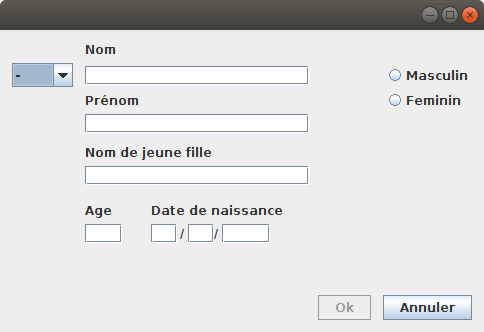
\includegraphics{images/dialogue.png}


\medskip

Vous pouvez ajouter des champs de saisie à votre gré, par exemple :
 \medskip

\begin{itemize}
% \item des champs de saisie de texte pour le nom, le prénom, le nom de jeune fille, l'âge, la date de naissance,
% \item une boîte à liste pour choisir entre Mlle, Mme ou M,
% \item des cases à cocher pour préciser le genre, masculin ou féminin,
\item des cases à cocher pour préciser le genre, majeur ou mineur,
\item des boutons \og radio \fg{} pour la situation matrimoniale, veuf (ou veuve), marié(e), divorcé(e), célibataire.
% \item deux boutons, ok et annuler, pour valider ou non la saisie.
\end{itemize}


\end{document}